%%%%%%%%%%%%%%%%%%%%%%%%%%%%%%%%%%%%%%%%%%%%%%%%%%%%%%%%%%%%%%%%%%%%%%%%%%%%%%%%%%%%%%%%%%%%%%%%
%
% CSCI 1430 Written Question Template
%
% This is a LaTeX document. LaTeX is a markup language for producing documents.
% Your task is to answer the questions by filling out this document, then to
% compile this into a PDF document.
%
% TO COMPILE:
% > pdflatex thisfile.tex
%
% If you do not have LaTeX and need a LaTeX distribution:
% - Departmental machines have one installed.
% - Personal laptops (all common OS): http://www.latex-project.org/get/
%
% If you need help with LaTeX, come to office hours. Or, there is plenty of help online:
% https://en.wikibooks.org/wiki/LaTeX
%
% Good luck!
% James and the 1430 staff
%
%%%%%%%%%%%%%%%%%%%%%%%%%%%%%%%%%%%%%%%%%%%%%%%%%%%%%%%%%%%%%%%%%%%%%%%%%%%%%%%%%%%%%%%%%%%%%%%%
%
% How to include two graphics on the same line:
%
% \includegraphics[width=0.49\linewidth]{yourgraphic1.png}
% \includegraphics[width=0.49\linewidth]{yourgraphic2.png}
%
% How to include equations:
%
% \begin{equation}
% y = mx+c
% \end{equation}
%
%%%%%%%%%%%%%%%%%%%%%%%%%%%%%%%%%%%%%%%%%%%%%%%%%%%%%%%%%%%%%%%%%%%%%%%%%%%%%%%%%%%%%%%%%%%%%%%%

\documentclass[11pt]{article}

\usepackage[english]{babel}
\usepackage[utf8]{inputenc}
\usepackage[colorlinks = true,
            linkcolor = blue,
            urlcolor  = blue]{hyperref}
\usepackage[a4paper,margin=1.5in]{geometry}
\usepackage{stackengine,graphicx}
\usepackage{fancyhdr}
\setlength{\headheight}{15pt}
\usepackage{microtype}
\usepackage{times}
\usepackage[shortlabels]{enumitem}
\setlist[enumerate]{topsep=0pt}
% python code format: https://github.com/olivierverdier/python-latex-highlighting
\usepackage{pythonhighlight}
\definecolor{lightgray}{RGB}{230,230,230}

\frenchspacing
\setlength{\parindent}{0cm} % Default is 15pt.
\setlength{\parskip}{0.3cm plus1mm minus1mm}

\pagestyle{fancy}
\fancyhf{}
\lhead{Homework on Scene Recognition: Written Questions}
\rhead{CSCI 1430}
\lfoot{\textcolor{red}{Only 
\ifcase\thepage
\or instructions
\or A1
\or A1
\or A2
\or A2
\or Q3
\or A3
\or A4
\or A5
\or Q6
\or A6
\or Q7
\or Q7
\or A7
\or feedback
\else
EXTRA PAGE ADDED
\fi
should be on this page
}}
\rfoot{\thepage~/ 13}

\date{}

\title{\vspace{-2cm}Scene Recognition Questions}


\begin{document}
\maketitle
\thispagestyle{fancy}
\vspace{-3cm}

\section*{Instructions}
\begin{itemize}
  \item 2 socially-responsible computing questions, which will be expanded on in discussion sections.
  \item 5 technical questions.
  \item Write code where appropriate; feel free to include images or equations.
  \item Please make this document anonymous.
  \item This assignment is \textbf{fixed length}, and the pages have been assigned for you in Gradescope. As a result, \textbf{please do NOT add any new pages}. We will provide ample room for you to answer the questions. If you \emph{really} wish for more space, please add a page \emph{at the end of the document}.
  \item \textbf{We do NOT expect you to fill up each page with your answer.} Some answers will only be a few sentences long, and that is okay.
\end{itemize}
\pagebreak

\paragraph{Q1:} The performance of trained classifiers is determined by the data we train them upon, and our perception of that performance is determined by how we evaluate them. One concern is that evaluation using overall accuracy can mask poor performance in specific subgroups caused by dataset bias.

Buolamwini and Gebru's 2018 paper \href{http://proceedings.mlr.press/v81/buolamwini18a/buolamwini18a.pdf}{Gender Shades: Intersectional Accuracy Disparities in Commercial Gender Classification} found that Microsoft's Face API trained gender classifier achieved 94\% overall accuracy, with 100\% accuracy on lighter-skinned male faces and 79.2\% accuracy on darker-skinned female faces. In response to the report, Microsoft \href{https://blogs.microsoft.com/ai/gender-skin-tone-facial-recognition-improvement/}{significantly improved} their classifier's performance. This occurred through ``expanded and revised training and benchmark datasets, new data collection efforts to further improve the training data by focusing specifically on skin tone, gender and age, and an improved classifier to produce higher precision results.'' These steps helped, but in general it is impossible to completely mitigate all bias in a real-world dataset. 

In this homework, we will train a scene recognition classifier using data from Lazebnik et al. 2006. Please review the data to check for potential biases: look at images in the data/train and data/test directories and consider their class labels. 

Please list at least three potential biases in the dataset, and describe a potential consequence for each for an application that trained with this data.

For example, if the street images in the dataset were used to train a pedestrian detector for a self-driving car, variation in clothing styles between training data and deployment environments might bias the classifier and fail to detect people. [1--2 sentences each]

\paragraph{A1:} Your answer here

\pagebreak

\textbf{Extra Space}

\pagebreak
 
\paragraph{Q2:}  It can be hard and expensive to find and collect data. One approach that researchers and companies have used is Web scraping, which downloads data across many websites to more easily create large datasets.

Web scraping has come under increasing scrutiny as computer vision systems have been deployed in real-world applications, because the technical capability to download publicly-accessible data does not imply consent for the use of that data. In 2021, France found that Clearview AI, a company that operates a facial recognition platform for law enforcement, \href{https://techcrunch.com/2021/12/16/clearview-gdpr-breaches-france/}{violated privacy laws} by scraping 10 billion images of people's faces from Facebook, YouTube, and other websites without consent.

a) How was the Lazebnik et al. 2006 dataset collected?

Dataset collection might merge multiple sources to fill in gaps in sampling a data distribution. Please find additional scene data that could be added to the Lazebnik et al. 2006 dataset. Here are two places to find datasets: \href{https://datasetsearch.research.google.com}{Google} and \href{https://www.kaggle.com}{Kaggle}. 

b) Find a dataset and provide a URL to it. Given your answers to Q1, describe how the new data addresses gaps in the project dataset and any limitations of the new data. [3--4 sentences] 

c) How was this new data collected? If you had to collect new scene data yourself, how would you do it? [6--7 sentences]

\paragraph{A2:} 

a) Your answer here

b) Your answer here

c) Your answer here

 

%%%%%%%%%%%%%%%%%%%%%%%%%%%%%%%%%%%
\pagebreak

\textbf{Extra Space}

\pagebreak

\paragraph{Q3:} 

\begin{enumerate} [(a)]
    \item Define these common terms in machine learning:
    \begin{enumerate} [(i)]
    \item Bias
    \item Variance
    \end{enumerate}
    \item Define these terms in the context of evaluating a classifier:
    \begin{enumerate} [(i)]
    \item Overfitting
    \item Underfitting
    \end{enumerate}
    \item How do overfitting and underfitting relate to bias and variance?
\end{enumerate}

\emph{Please answer on the next page.}

%%%%%%%%%%%%%%%%%%%%%%%%%%%%%%%%%%%
\pagebreak
\paragraph{A3:} Your answer here.
% Uncomment the stencil below and fill in your solution.

% \begin{enumerate}[(a)]

% \item 
%     \begin{enumerate} [(i)]
%     \item 
%     \item
%     \end{enumerate}

% \item 
%     \begin{enumerate} [(i)]
%     \item 
%     \item
%     \end{enumerate}
% \item 

% \end{enumerate}


%%%%%%%%%%%%%%%%%%%%%%%%%%%%%%%%%%%

\pagebreak
\paragraph{Q4:} Suppose we create a visual word dictionary using SIFT and k-means clustering for a scene recognition algorithm. Examining the SIFT features generated from our training database, we see that many are almost equidistant from two or more visual words. 
\begin{enumerate}[(a)]
    \item 
    Why might this affect classification accuracy?

    \item
    Given the situation, describe \emph{two} methods to improve classification accuracy, and explain why they would help.\\ 
    \emph{These can be for k-means, or otherwise.}

\end{enumerate}


%%%%%%%%%%%%%%%%%%%%%%%%%%%%%%%%%%%
\paragraph{A4:} Your answer here.
% Uncomment the stencil below and fill in your solution.

% \begin{enumerate}[(a)]

% \item 

% \item 

% \end{enumerate}



%%%%%%%%%%%%%%%%%%%%%%%%%%%%%%%%%%%

\pagebreak
\paragraph{Q5:} The way that the bag of words representation handles the spatial layout of visual information can be both an advantage and a disadvantage.
\begin{enumerate}[(a)]
\item Describe an example scenario for each of these cases.
\item Describe a modification or additional algorithm which might\\overcome the disadvantage.

\item How might we determine whether bag of words is a good model?
\end{enumerate}
%%%%%%%%%%%%%%%%%%%%%%%%%%%%%%%%%%%
\paragraph{A5:} Your answer here.
% Uncomment the stencil below and fill in your solution.

% \begin{enumerate}[(a)]

% \item 

% \item 

% \item 

% \end{enumerate}




%%%%%%%%%%%%%%%%%%%%%%%%%%%%%%%%%%%

\pagebreak
\paragraph{Q6:} Given a linear classifier such as SVM which separates two classes (binary decision), how might we use multiple linear classifiers to create a new classifier which separates $k$ classes?

Below, we provide pseudocode for a linear classifier. It trains a model on a training set, and then classifies a new test example into one of two classes. Please edit the pseudo-code to convert this into a multi-class classifier. 

\emph{Hints:} See slides in supervised learning crash course deck, plus your own research. You can take either the one vs.~all (or one vs.~others) approach or the one vs.~one approach in the slides; please declare which approach you take.

\emph{More hints:} Be aware that:
\begin{enumerate}
    \item The input labels in the multi-class case are different, and you will need to match the expected label input for the \texttt{train\_linear\_classifier} function
    \item You need to make a new decision on how to aggregate or decide on the most confident prediction
\end{enumerate}

\emph{Note:} A more efficient software application would separate the classifier training and testing into two different functions so that the model could be reused without retraining. Feel free to ignore this for now.

\emph{Please answer on the next page.}

%%%%%%%%%%%%%%%%%%%%%%%%%%%%%%%%%%%
\pagebreak
\paragraph{A6:} Your answer here.

\begin{python}
# Inputs
#   train_feats: N x d matrix of N features each d descriptor long
#   train_labels: N x 1 array containing values of either -1 
#               (class 0) or 1 (class 1)
#   test_feat: 1 x d image for which we wish to predict a label
#
#   Outputs: -1 (class 0) or 1 (class 1)
#
# Please turn this into a multi-class classifier for k classes.
# Inputs:
#    As before, except
#    train_labels: N x 1 array of class label integers from 0 to k-1
# Outputs:
#    A class label integer from 0 to k-1
#
def classify(train_feats, train_labels, test_feat)
    # Train classification hyperplane
    weights, bias = train_linear_classifier(train_feats, train_label)
    # Compute distance from hyperplane
    test_score = weights * test_feats + bias

    return 1 if test_score > 0 else -1
\end{python}
% %%%%%%%%%%%%%%%%%%%%%%%%%%%%%%%%%%%


% %%%%%%%%%%%%%%%%%%%%%%%%%%%%%%%%%%%
\pagebreak

\paragraph{Q7:} In this homework, we will use a feature descriptor called HOG---`Histogram of Oriented Gradients'. As its name implies, it works similarly to SIFT. In classification, we might extract HOG features across the entire image (not just at corners) to create visual words.

HOG creates a feature descriptor per image `block'. Each block is split into `cells' covering pixels. HOG outputs a 9-bin histogram of oriented gradients per cell. We append these together to obtain the feature descriptor for each block. As a result, if we have $(z,z)$ cells per block, the feature descriptor for each block will be of size $z \times z \times 9$. 

\emph{Blocks can overlap as displayed in the diagram below.}
%
\begin{center}
    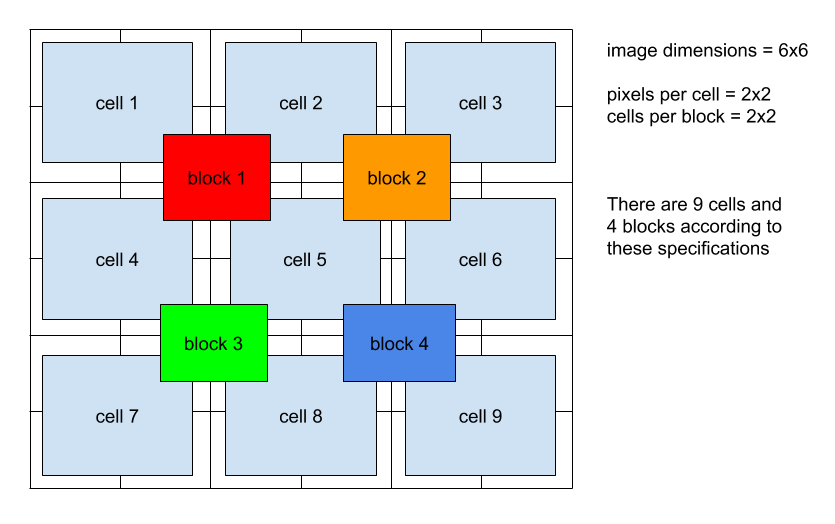
\includegraphics[clip, trim = {0.2cm, 0.35cm, 0.2cm, 0.2cm}, width=12.5cm]{hog-diagram.png} % 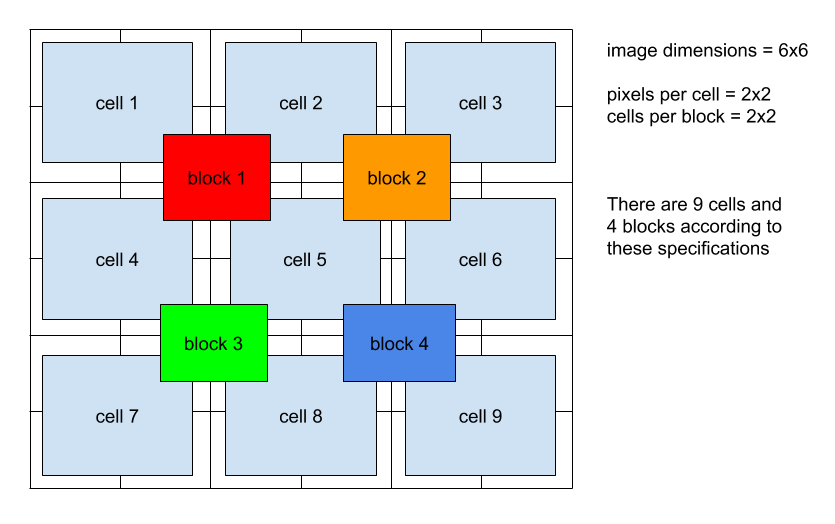
\includegraphics[clip,trim={0cm 0.75cm 0cm 0.75cm},width=11cm]{hog-diagram.png}
\end{center}
%
When using HOG, the parameters such as pixels per cell and cells per block impact the resulting feature descriptor and so our performance on a classification task.

\begin{enumerate}[(a)]
\item Given a \colorbox{lightgray}{$72\times72$} image, calculate the number of cells, blocks, and feature vector size that will occur when we extract HOG features with the following parameters using maximum overlap between blocks.

Scenario 1: Pixels per cell = \colorbox{lightgray}{$4\times4$}, cells per block = \colorbox{lightgray}{$4\times4$} % (\emph{like in SIFT!}). 
\\
\emph{Calculate:}
\\ 
Number of cells: 
\\
Number of blocks: 
\\
Dimensions of resulting feature descriptor: 
\\

Scenario 2: Pixels per cell = \colorbox{lightgray}{$8\times8$}, cells per block = \colorbox{lightgray}{$2\times2$}.
\\
\emph{Calculate:}
\\ 
Number of cells:
\\
Number of blocks: 
\\
Dimensions of resulting feature descriptor: 


\item What are the pros and cons of the two parameter combinations? Which might you expect to have better performance?

\emph{Note: You may find it useful to look at the thesis of Navneet Dalal (co-inventor of HOG) for more on this topic. \href{http://lear.inrialpes.fr/people/dalal/NavneetDalalThesis.pdf}{[Link to thesis]} (pages 39, 41 in Section 4.3).}

\end{enumerate}

\emph{Please answer on the next page.}


%%%%%%%%%%%%%%%%%%%%%%%%%%%%%%%%%%%
\pagebreak
\paragraph{A7:} Your answer here.
% Uncomment the stencil below and fill in your solution.

% a)
% Scenario 1:
% \\ 
% Number of cells: 
% \\
% Number of blocks: 
% \\
% Dimensions of resulting feature descriptor: 
% \\


% Scenario 2:
% \\ 
% Number of cells: 
% \\
% Number of blocks: 
% \\
% Dimensions of resulting feature descriptor: 
% \\


% What are the pros and cons of the two parameter combinations? Which might you expect to have better performance?
% 

%%%%%%%%%%%%%%%%%%%%%%%%%%%%%%%%%%%



% %%%%%%%%%%%%%%%%%%%%%%%%%%%%%%%%%%%
% \pagebreak
% \paragraph{Secret something to think about:} Given a linear classifier like SVM, how might we handle data that are not linearly separable? How does the \emph{kernel trick} help in these cases? 

% \emph{Hint: See slides in supervised learning crash course deck, plus your own research.}

% %%%%%%%%%%%%%%%%%%%%%%%%%%%%%%%%%%%
% \paragraph{A:} Your answer here.



%%%%%%%%%%%%%%%%%%%%%%%%%%%%%%%%%%%
\pagebreak
\section*{Feedback? (Optional)}
Please help us make the course better. If you have any feedback for this assignment, we'd love to hear it!


% \pagebreak
% \section*{Any additional pages would go here.}


\end{document}
